\documentclass[twoside,11pt]{article}

\usepackage{amsmath}
\usepackage{booktabs}
\usepackage{multirow}
\usepackage{jmlr2e}
\hypersetup{colorlinks=true, urlcolor=blue, citecolor=blue, linkcolor=blue}

\usepackage{lastpage}
\jmlrheading{0}{2026}{1-\pageref{LastPage}}{5/26}{}{stats-signals-01}{Aksel Kretsinger-Walters}

\ShortHeadings{GLRT Detection of Timeout Effects in the NBA}{Aksel Kretsinger-Walters}
\firstpageno{1}

\begin{document}

\title{Detecting Timeout Effects in the NBA via the Generalized Likelihood Ratio Test}

\author{\name Aksel Kretsinger-Walters \email adk2164@columbia.edu \\
		\addr Department of Computer Science\\
		Columbia University\\
New York, NY 10027, USA}

\editor{}

\maketitle

\begin{abstract}%
		We frame the question ``does an NBA timeout move the game?'' as a battery of
		one-sample Gaussian signal-detection problems. For three impact metrics
		derived from the cdnnba 2020--2025 play-by-play feed---excess net points,
		excess points-per-possession, and win-probability added---we test
		$H_0\!:\mu = 0$ against $H_1\!:\mu \neq 0$ via the generalized likelihood
		ratio statistic $G = -2\log\Lambda$, which under $H_0$ is asymptotically
		$\chi^2_1$. The three metrics are evaluated separately for coach full
		timeouts, coach challenges, and inferred mandatory television timeouts, and
		within each subtype we stratify by score margin, streak, game phase, home
		court, and regular season vs.\ playoffs. The point-differential metric
		collapses to a null result aggregated, but reveals a structured
		regression-to-mean signal once stratified by margin or streak. The
		win-probability metric rejects $H_0$ overwhelmingly: full timeouts cost the
		calling team roughly $3.9$ percentage points of WP across a $\pm 6$
		possession window, challenges add roughly $1.6$ pp, and television timeouts
		cost $1.3$ pp---a pattern consistent with the prior causal literature.
		Across $163$ stratified GLRTs, we reject $H_0$ in $69$ cases ($42.3\%$),
		versus the $\sim$$5\%$ expected if the null held everywhere.
\end{abstract}

\begin{keywords}
		Generalized likelihood ratio test, signal detection, sports analytics, NBA,
		timeouts, win probability
\end{keywords}

\section{Problem Statement}
\label{sec:problem}

The NBA play-by-play feed records, for every coach-called timeout, the game
state immediately before and after the stoppage. Whether timeouts actually
``do something'' to the game is contested in the literature
\citep{assis2020stop,gibbs2021causal,weimer2023causal,qiu2025interrupt}.
We treat each of three derived per-event impact metrics as a sample from a
real-valued source and ask the binary signal-detection question
``is the source mean zero?''

Concretely, let $X_1,\dots,X_n$ be the impact-metric values across timeouts
within some stratum (e.g.\ full coach timeouts called while leading by
6--15 points), modeled as iid $\mathcal{N}(\mu, \sigma^2)$ with both
parameters unknown. We test
\begin{equation}
		H_0\!: \mu = 0 \qquad \text{vs.} \qquad H_1\!: \mu \neq 0.
		\label{eq:hyp}
\end{equation}
A rejection means the timeout type, conditioned on the stratum, is
associated with a non-zero shift in the metric.

\section{Data and Metrics}
\label{sec:data}

We use the cdnnba enriched play-by-play feed for the 2020--2025 NBA seasons
(regular season and playoffs), spanning $4{,}183{,}347$ rows across
$7{,}457$ games and $1{,}480{,}697$ possessions. Mandatory television
timeouts are not labeled in the feed; we inject them via a deterministic
rulebook procedure validated against the explicitly labeled 2013--2016
nbastatsv3 feed (F1 $= 0.88$--$0.92$). After injection, the cdnnba era
contains $74{,}236$ \texttt{full} coach timeouts, $1{,}396$ \texttt{challenge}
events, and $14{,}538$ inferred \texttt{official\_inferred} (TV) timeouts.

For each timeout event we look at a window of $W=6$ possessions before and
$W$ after, and compute three metrics from the calling team's perspective.
\begin{description}
		\item[Q1.~\texttt{excess\_net\_post}] Calling-team net points (for--against)
				in the post window, minus the season-PPP-gap expectation
				$(\mathrm{PPP}_{\text{calling}} - \mathrm{PPP}_{\text{opponent}})\cdot W/2$.
				$\mu = 0$ corresponds to the calling team performing at the season expectation.
		\item[Q2.~\texttt{excess\_ppp\_for\_post}] Calling-team PPP in the post window
				minus that team's full-season PPP. $\mu = 0$ means the team scores at
				season pace.
		\item[Q3.~\texttt{wp\_added\_calling}] Change in calling-team win probability
				across the $\pm W$ possession window, where $\Pr(\text{home wins})$ is the
				output of a logistic-regression model trained on possession-start snapshots
				with the ten features score margin, period, seconds remaining,
				clutch indicator, possessing-team-is-home indicator, streak,
				playoff indicator, home win-percentage, away win-percentage, and the
				home-minus-away win-percentage difference. $\mu = 0$ means
				the window had no net WP movement for the calling team.
\end{description}
The WP model achieves AUC $0.844$ and Brier score $0.161$ on a
held-out-by-game test set ($n=59{,}860$).

For each metric we run the GLRT separately for the three timeout subtypes
and stratify on five context columns from the project README:
\texttt{is\_home\_calling}, \texttt{IsPlayoff}, \texttt{time\_bucket}
($\text{Q1}, \text{Q2}, \text{Q3}, \text{Q4\_early}, \text{Q4\_clutch},
\text{OT}$), \texttt{margin\_bucket} (seven buckets from down-15 to up-15
from the calling team's perspective), and \texttt{streak\_bucket} (seven
buckets from a 10-pt opposing run to a 10-pt own run).

\section{Methods: GLRT Derivation}
\label{sec:method}

For $X_1,\dots,X_n$ iid $\mathcal{N}(\mu, \sigma^2)$ the log-likelihood is
\[
		\log L(\mu, \sigma^2) = -\tfrac{n}{2}\log(2\pi\sigma^2) -
		\frac{1}{2\sigma^2}\sum_{i=1}^n (x_i - \mu)^2.
\]
Under $H_0$ ($\mu=0$) the MLE is $\hat\sigma^2_0 = \tfrac{1}{n}\sum x_i^2$;
under $H_1$ the MLEs are $\hat\mu_1 = \bar x$ and $\hat\sigma^2_1 =
\tfrac{1}{n}\sum (x_i - \bar x)^2$. The supremum log-likelihood under each
hypothesis evaluates to $-\tfrac{n}{2}(1 + \log(2\pi\hat\sigma^2_*))$, so
the generalized likelihood ratio is
\begin{equation}
		\Lambda \;=\; \frac{\sup_{\sigma^2} L(0, \sigma^2)}
		{\sup_{\mu, \sigma^2} L(\mu, \sigma^2)}
		\;=\; \Big(\frac{\hat\sigma^2_1}{\hat\sigma^2_0}\Big)^{n/2}.
		\label{eq:lambda}
\end{equation}
Using the identity $\hat\sigma^2_0 = \hat\sigma^2_1 + \bar x^2$ we obtain
the test statistic
\begin{equation}
		G \;=\; -2\log\Lambda \;=\; n\,\log\!\Big(1 + \frac{\bar x^2}{\hat\sigma^2_1}\Big),
		\label{eq:glrt}
\end{equation}
which by Wilks' theorem is asymptotically $\chi^2_1$ under $H_0$. We reject
$H_0$ at level $\alpha = 0.05$ when $G > \chi^2_{1, 0.95} \approx 3.841$.
Equivalently, with $s^2 = \tfrac{n}{n-1}\hat\sigma^2_1$ and the one-sample
$t$-statistic $t = \bar x / (s/\sqrt n)$,
\[
		G = n\,\log\!\left(1 + \frac{t^2}{n - 1}\right) \;\xrightarrow{n\to\infty}\; t^2,
\]
so the GLRT and the standard $t$-test are asymptotically equivalent;
we report both throughout for cross-checking.

\section{Results}
\label{sec:results}

\subsection{Aggregated GLRT Results}

Table~\ref{tab:overall} reports the GLRT statistic for each
$(\text{metric}, \text{subtype})$ pair pooled over the entire cdnnba era.

\begin{table}[t]
		\centering
		\small
		\begin{tabular}{llrrrrl}
				\toprule
				Metric & Subtype & $n$ & $\bar x$ & $G$ & $p$ & sig.\ \\
				\midrule
				\multirow{3}{*}{Q1: excess net post}
				& full              & 74{,}236 & $-0.011$ & $0.98$    & $0.32$  & ns  \\
				& challenge         & 1{,}396  & $-0.112$ & $2.16$    & $0.14$  & ns  \\
				& official\_inferred& 14{,}538 & $-0.003$ & $0.01$    & $0.90$  & ns  \\
				\midrule
				\multirow{3}{*}{Q2: excess PPP for post}
				& full              & 74{,}236 & $+0.007$ & $7.12$    & $0.008$ & **  \\
				& challenge         & 1{,}396  & $-0.021$ & $1.42$    & $0.23$  & ns  \\
				& official\_inferred& 14{,}538 & $+0.013$ & $5.59$    & $0.018$ & *   \\
				\midrule
				\multirow{3}{*}{Q3: WP added (calling)}
				& full              & 74{,}236 & $-0.039$ & $10{,}881$ & $<10^{-300}$ & *** \\
				& challenge         & 1{,}396  & $+0.016$ & $34.3$    & $4.7\!\times\!10^{-9}$  & *** \\
				& official\_inferred& 14{,}538 & $-0.013$ & $245.2$   & $<10^{-50}$  & *** \\
				\bottomrule
		\end{tabular}
		\caption{Aggregated GLRT results by metric and timeout subtype.
				Significance: ns ($p \geq 0.05$), $*$ ($p < 0.05$), $**$ ($p < 0.01$),
		$***$ ($p < 0.001$).}
		\label{tab:overall}
\end{table}

\paragraph{Q1.} Pooled over the league, the calling team's net post-window
points cannot be statistically distinguished from the season-PPP
expectation: $G = 0.98$, $p = 0.32$ for the most populous \texttt{full}
subtype. This is the canonical null result reported by
\citet{assis2020stop} and is consistent with the regression-to-the-mean
explanation: timeouts are most often called from a deficit, and the gap
between pre-timeout net ($\bar x_{\text{pre}} = -1.73$ pts) and
post-timeout net ($\bar x_{\text{post}} = -0.02$ pts) absorbs into the
season baseline once we subtract the PPP gap.

\paragraph{Q2.} The PPP metric---which removes the opponent's
contribution---rejects $H_0$ for both \texttt{full} ($+0.007$ PPP, $p =
0.008$) and \texttt{official\_inferred} ($+0.013$ PPP, $p = 0.018$).
The effect is small but real: full coach timeouts add about $0.7\%$ of a
possession's worth of scoring relative to the calling team's season
average, and TV timeouts add about $1.3\%$.

\paragraph{Q3.} The WP metric overwhelmingly rejects $H_0$ for every
subtype. Full timeouts cost the calling team an average of $3.9$ WP
percentage points across the $\pm 6$ possession window
($G = 1.09\!\times\!10^4$), challenges \emph{add} $1.6$ pp
($G = 34$, $p < 10^{-8}$), and TV timeouts cost $1.3$ pp ($G = 245$).
The challenge sign is intuitive---challenges are issued when a team
believes it has been wronged, so the post-window typically reflects a
restored possession or extra free throws---but the negative WP for full
coach timeouts is striking, and aligns with the slightly negative ATT
that \citet{gibbs2021causal} found via genetic matching.

Figure~\ref{fig:overall-three} shows the GLRT statistics on a log scale
alongside the sample mean with $95\%$ confidence intervals. The huge
spread between Q1 and Q3 visualizes the value of measuring impact in WP
units rather than in raw point swings.

\begin{figure}[t]
		\centering
		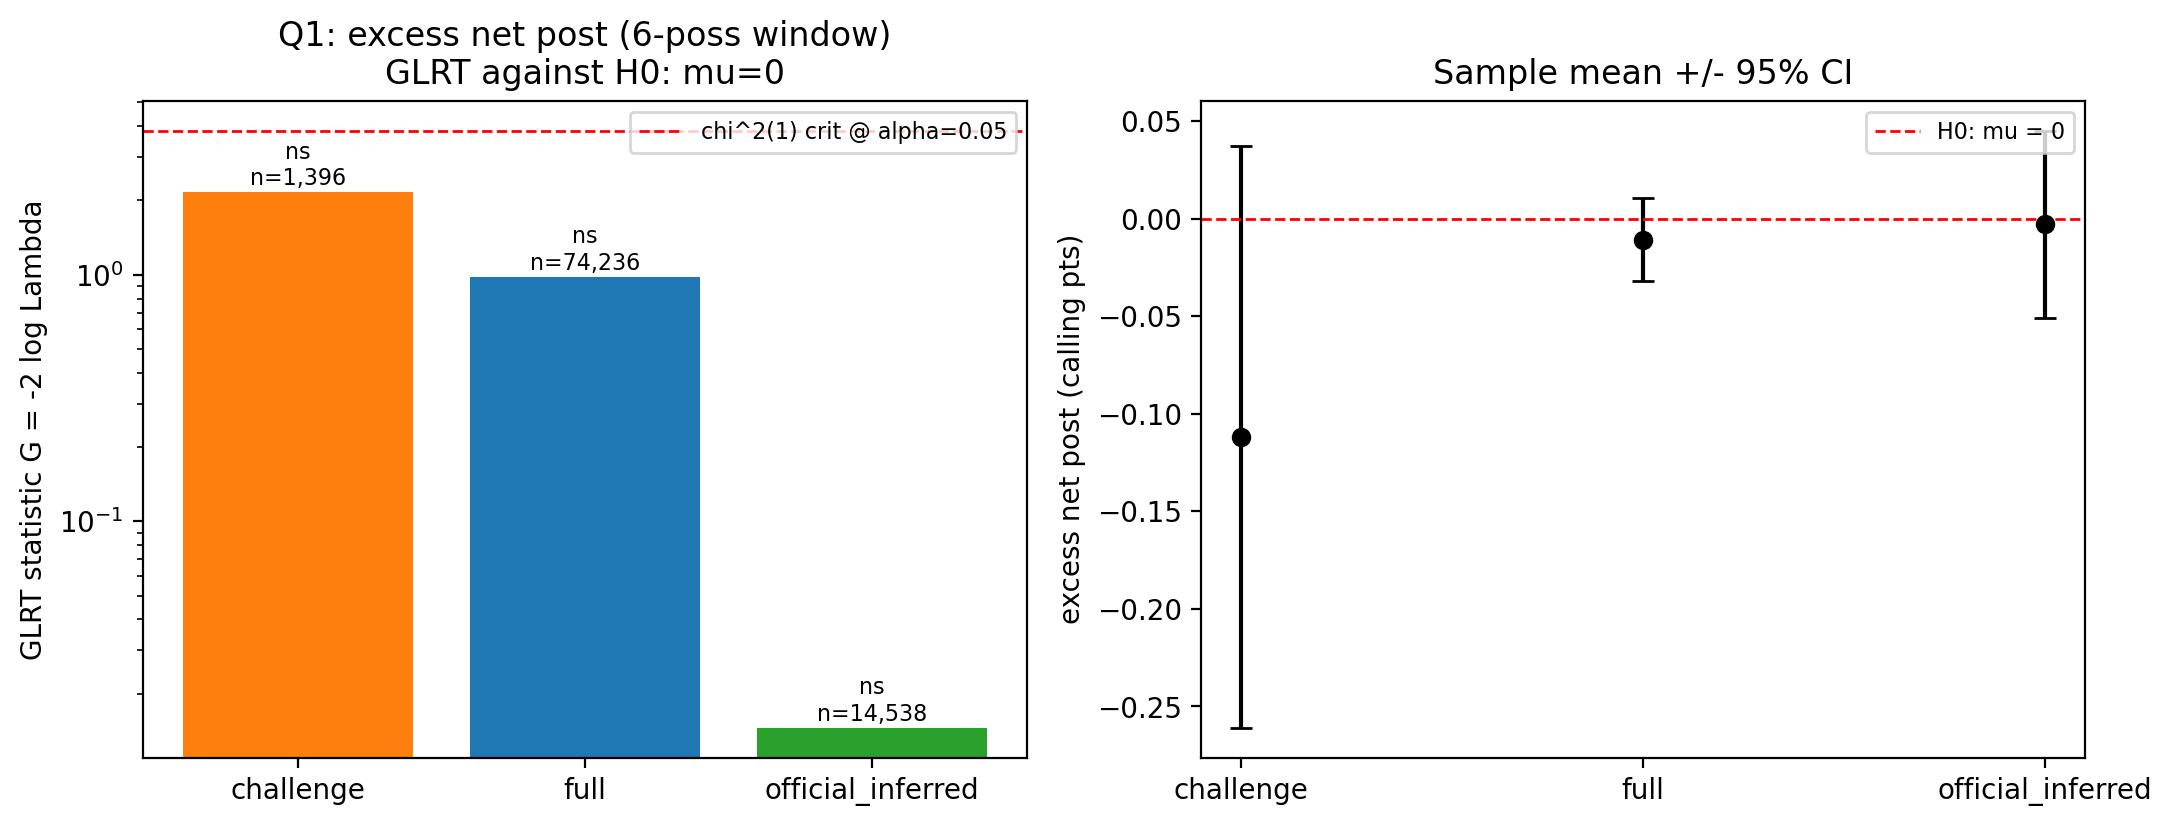
\includegraphics[width=0.32\textwidth]{figures/q1_overall.jpg}\hfill
		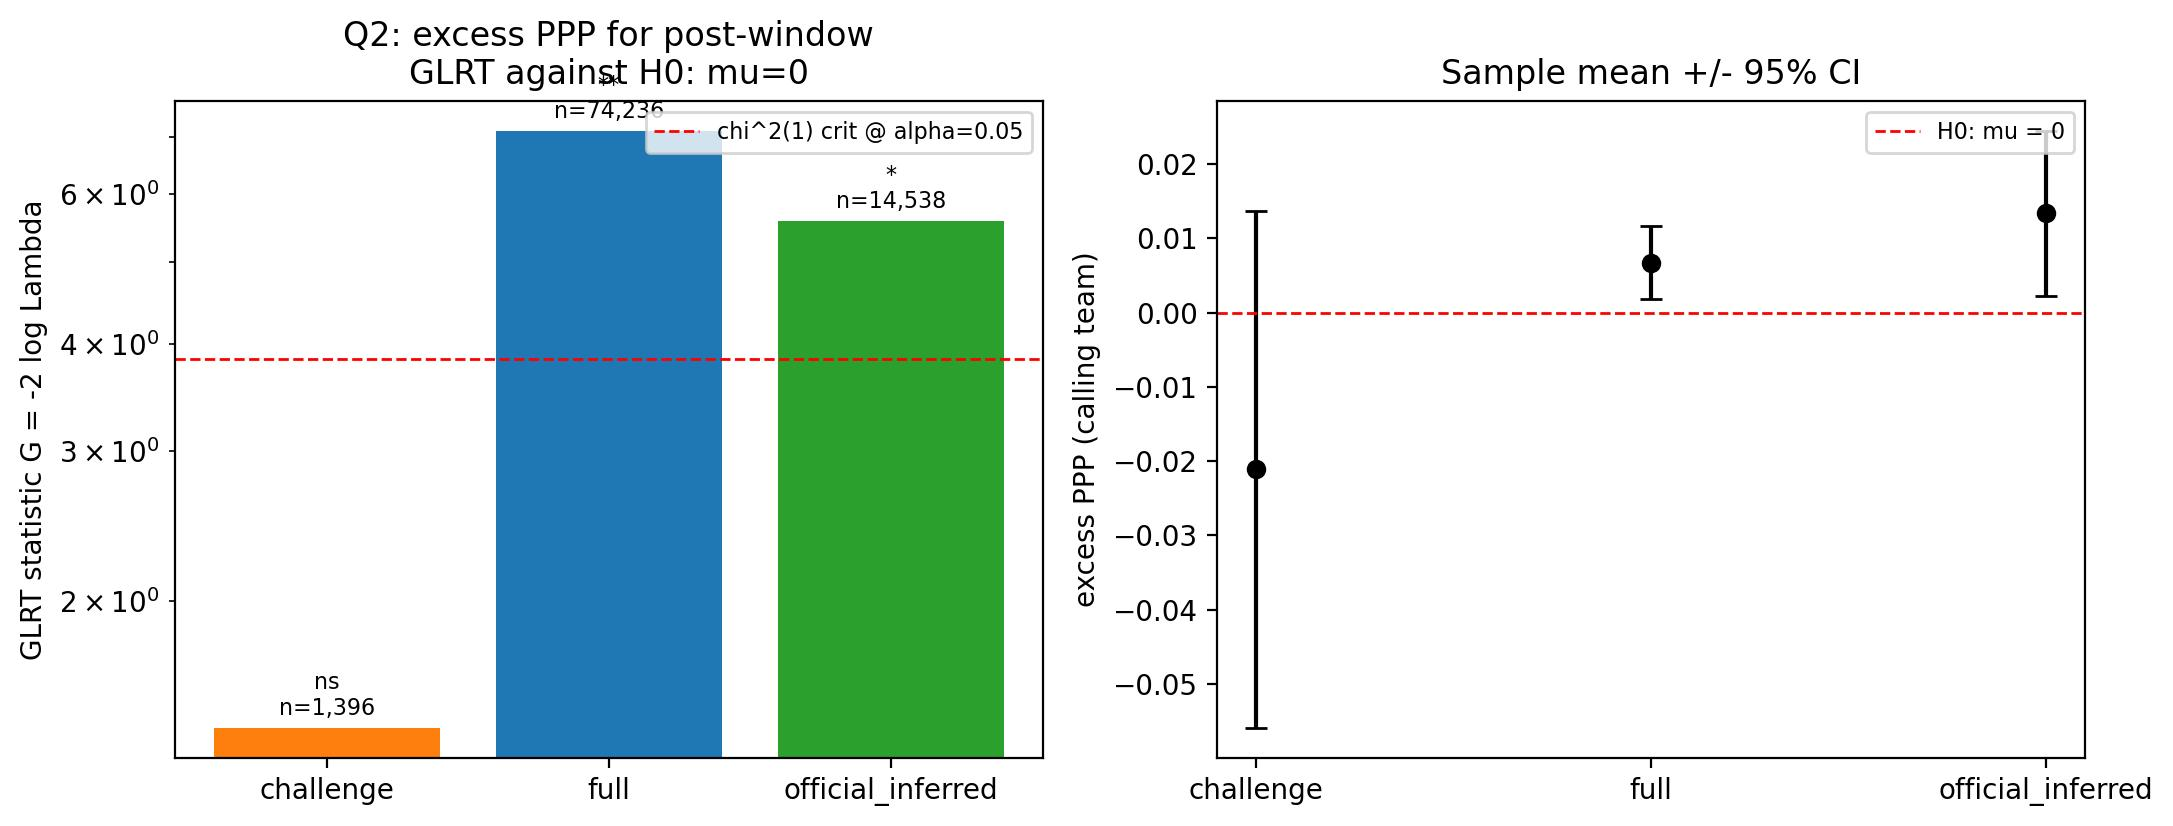
\includegraphics[width=0.32\textwidth]{figures/q2_overall.jpg}\hfill
		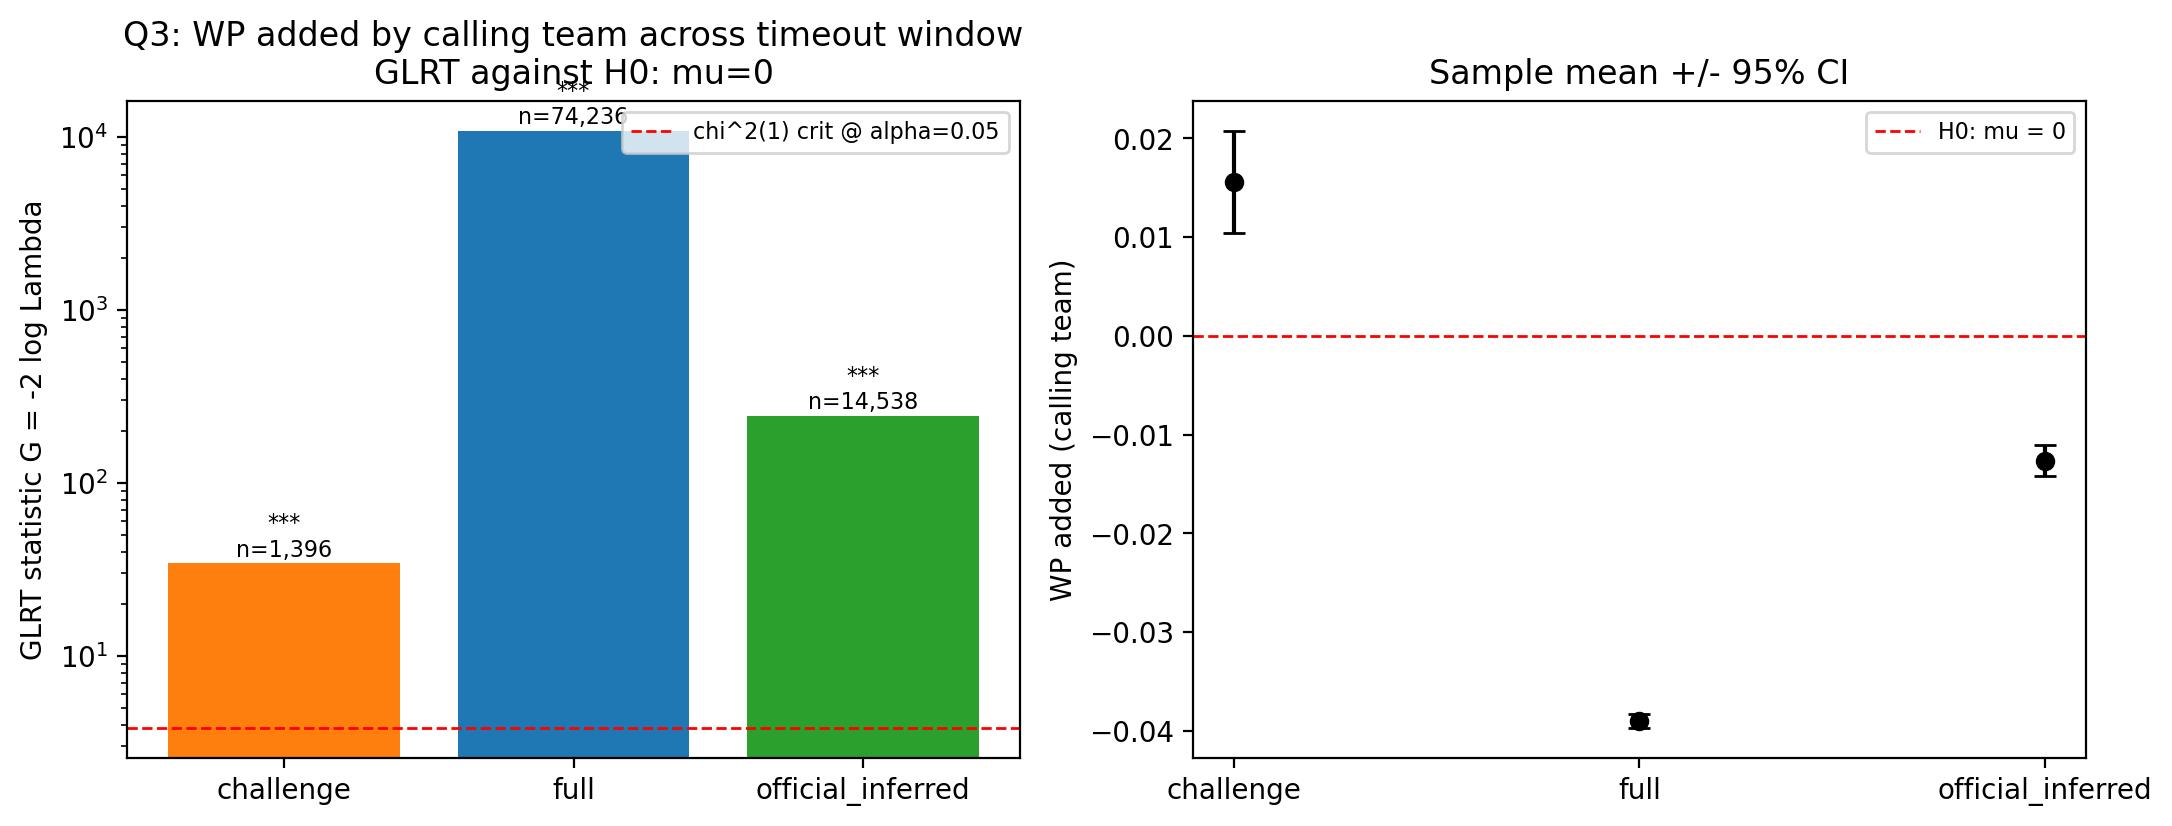
\includegraphics[width=0.32\textwidth]{figures/q3_overall.jpg}
		\caption{Aggregated GLRT statistics and means for Q1 (left), Q2
				(middle), and Q3 (right). The dashed red line on the left panel of
		each plot is $\chi^2_{1,0.95} = 3.841$.}
		\label{fig:overall-three}
\end{figure}

\subsection{Stratified by Pre-Timeout Streak}

The streak bucket categorizes the calling team's signed streak (positive
when the calling team itself has been on a run). Figure~\ref{fig:q3-streak}
shows that the WP signal is highly heterogeneous: timeouts called \emph{into}
a $6$--$9$-point opposing run cost the full-timeout caller $-10.3$ pp of
WP ($G = 12{,}992$, $n = 15{,}219$); timeouts called while the calling team
itself is on a $6$--$9$-point run \emph{add} $+9.5$ pp ($G = 1{,}135$,
$n = 1{,}470$). Crucially, the magnitude of the signed effect is roughly
symmetric around streak $= 0$: timeouts do not appear to reverse momentum
within the post window---they appear to ride it, regardless of which side
the timeout was called from.

\begin{figure}[t]
		\centering
		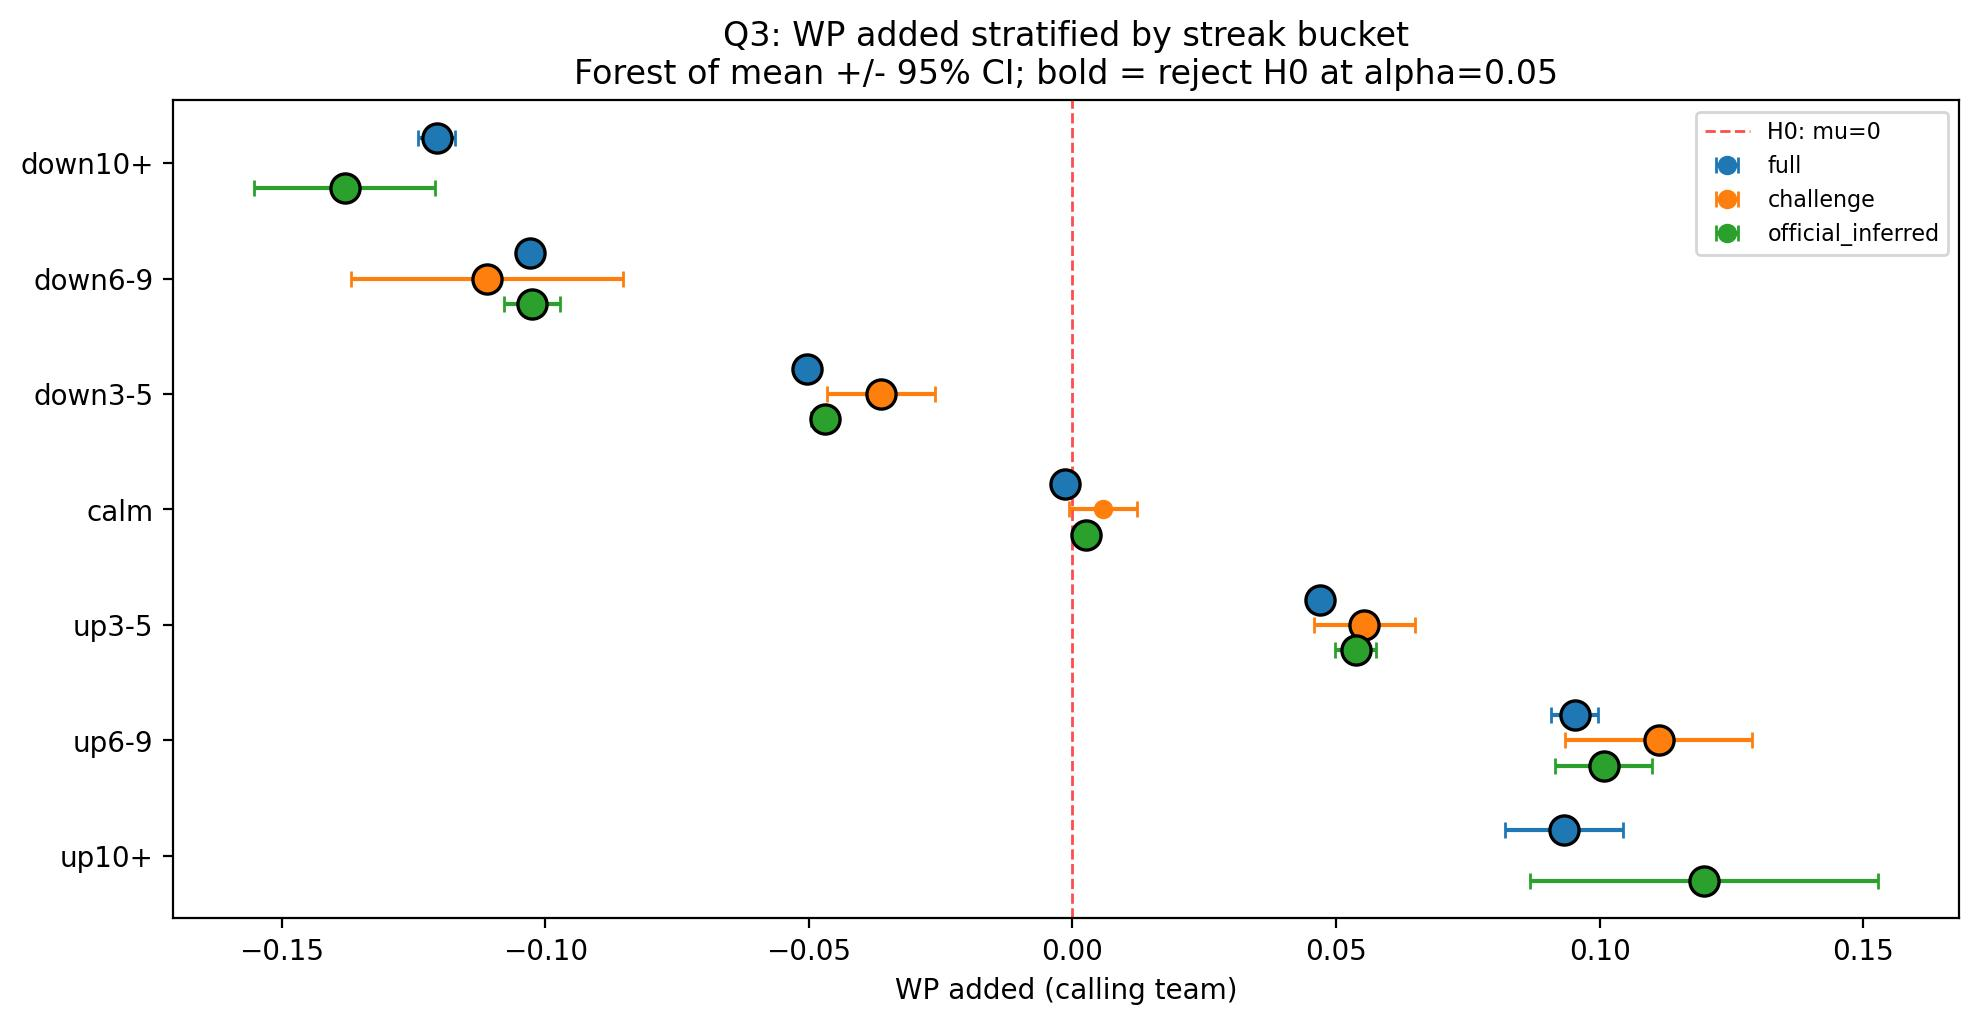
\includegraphics[width=0.85\textwidth]{figures/q3_streak.jpg}
		\caption{Q3 WP added stratified by pre-timeout streak. Bold filled markers
		indicate strata where $H_0\!:\mu=0$ is rejected at $\alpha = 0.05$.}
		\label{fig:q3-streak}
\end{figure}

The same stratification on Q1 (Figure~\ref{fig:q1-streak}) is far less
sharp---the signal is largely absorbed by the PPP-gap baseline---but the
direction matches: down-streak timeouts produce small positive Q1 excesses,
up-streak timeouts produce small negative ones.

\begin{figure}[t]
		\centering
		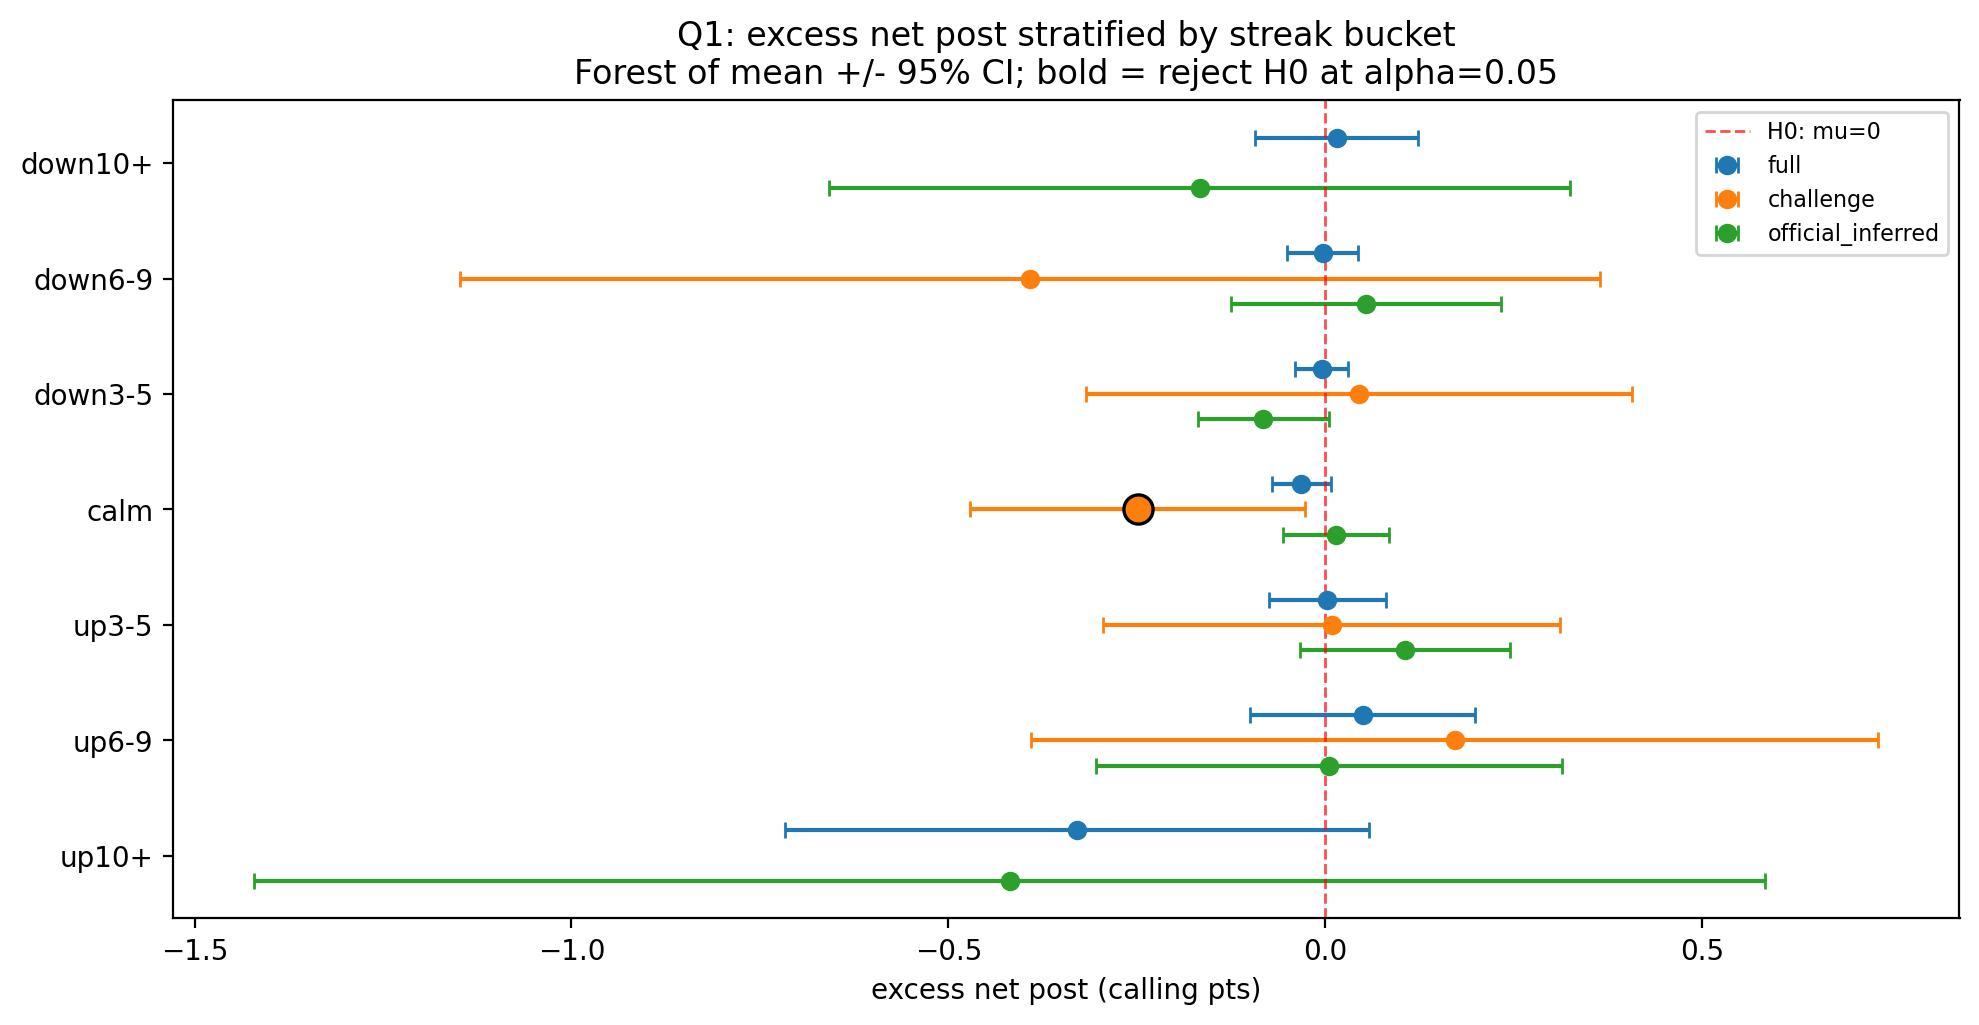
\includegraphics[width=0.85\textwidth]{figures/q1_streak.jpg}
		\caption{Q1 excess net post stratified by pre-timeout streak. Bold filled
		markers indicate strata where $H_0$ is rejected at $\alpha = 0.05$.}
		\label{fig:q1-streak}
\end{figure}

\subsection{Stratified by Score Margin}

Stratifying on the calling team's score margin
(Figure~\ref{fig:q1-margin}) exposes a very clean regression-to-mean
pattern in the point-differential metric that is hidden by aggregation.
For \texttt{full} timeouts, all three down-by buckets show positive Q1
excess (\texttt{down15+}: $+0.17$, $G = 24.4$; \texttt{down6-15}: $+0.11$,
$G = 24.9$) while all three up-by buckets show negative Q1 excess
(\texttt{up15+}: $-0.26$, $G = 39.5$; \texttt{up6-15}: $-0.16$,
$G = 37.8$). The same monotone pattern holds, weaker, for inferred TV
timeouts, but the challenge subtype shows no margin signal due to small
sample sizes.

\begin{figure}[t]
		\centering
		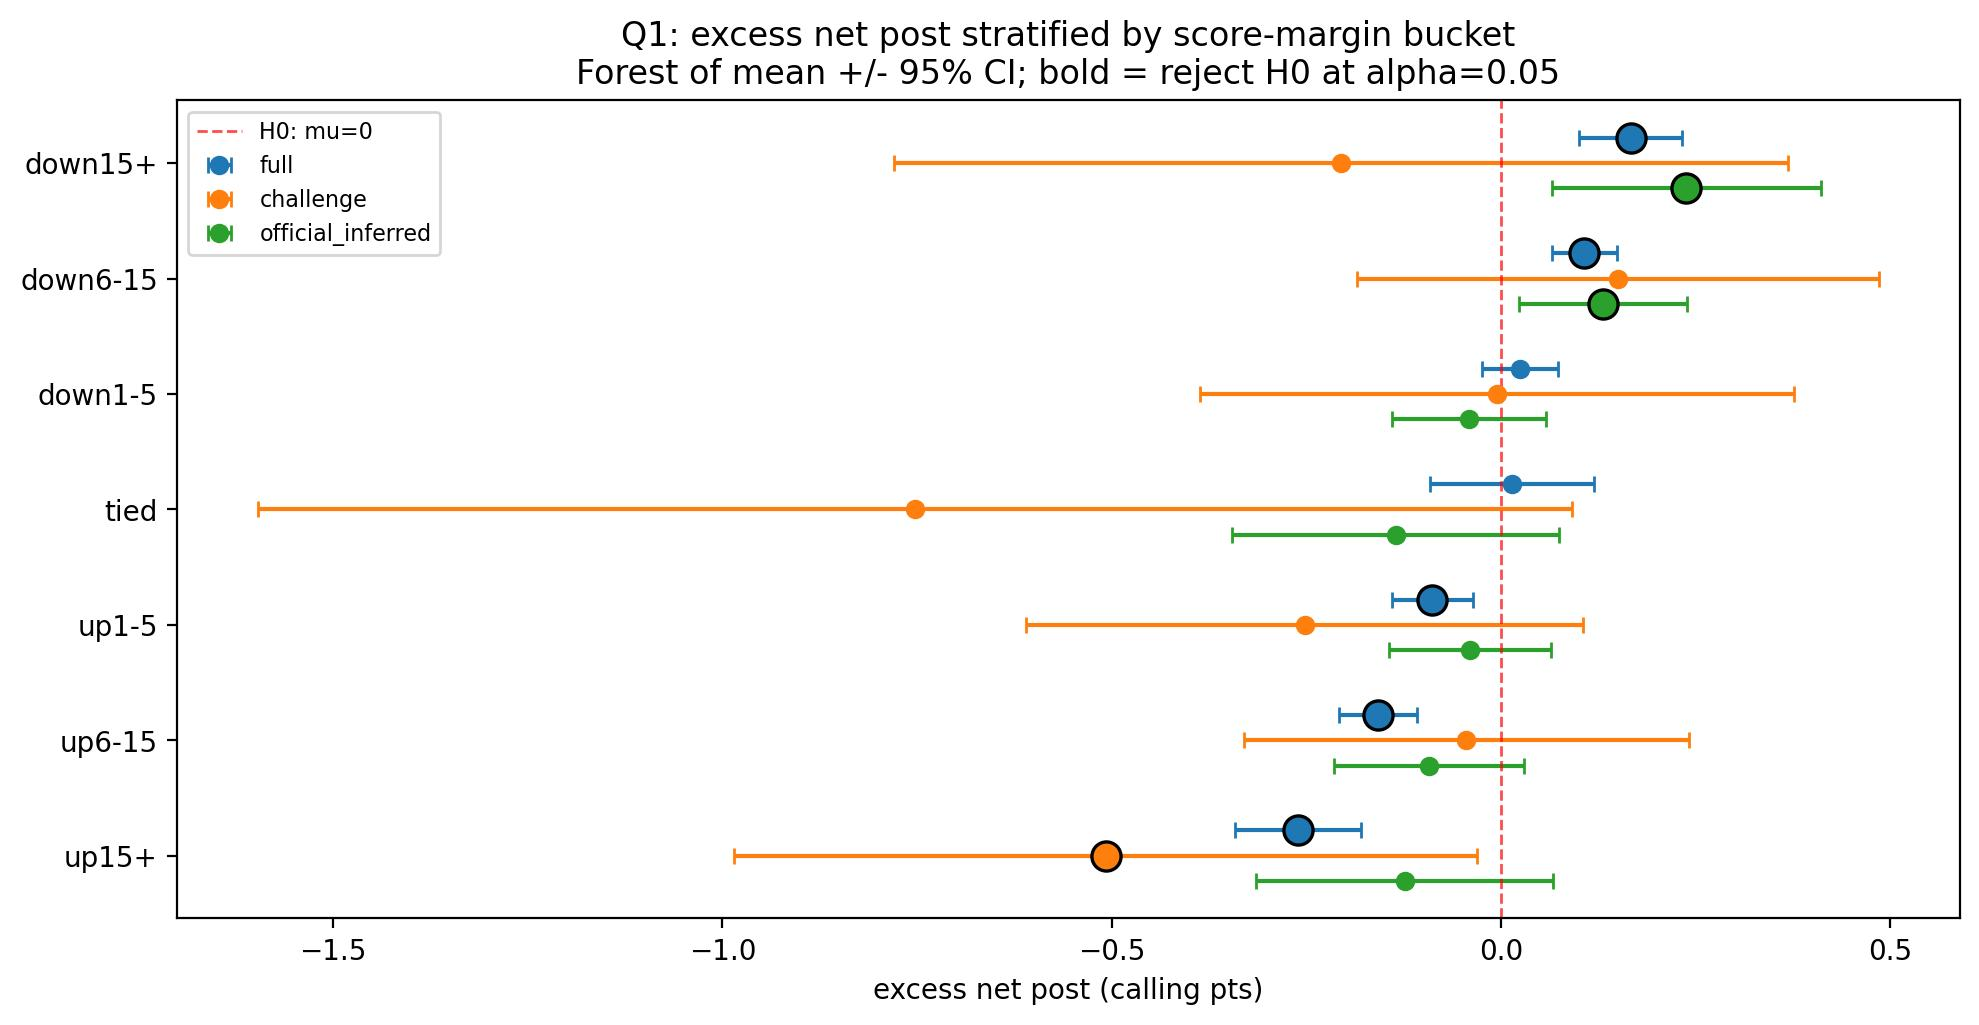
\includegraphics[width=0.85\textwidth]{figures/q1_margin.jpg}
		\caption{Q1 excess net post stratified by calling-team score margin. The
				left-to-right monotone trend is the regression-to-mean signature: trailing
				teams gain back roughly what they were missing, leading teams give some
		back.}
		\label{fig:q1-margin}
\end{figure}

The Q3 margin stratification (Figure~\ref{fig:q3-margin}) tells a
complementary story. Full-timeout WP loss is largest in moderately
adverse situations (\texttt{down6-15}: $-6.1$ pp, $G = 6{,}749$;
\texttt{down1-5}: $-5.3$ pp, $G = 2{,}562$) and shrinks toward zero in
extreme leads or deficits where the win is largely already decided.

\begin{figure}[t]
		\centering
		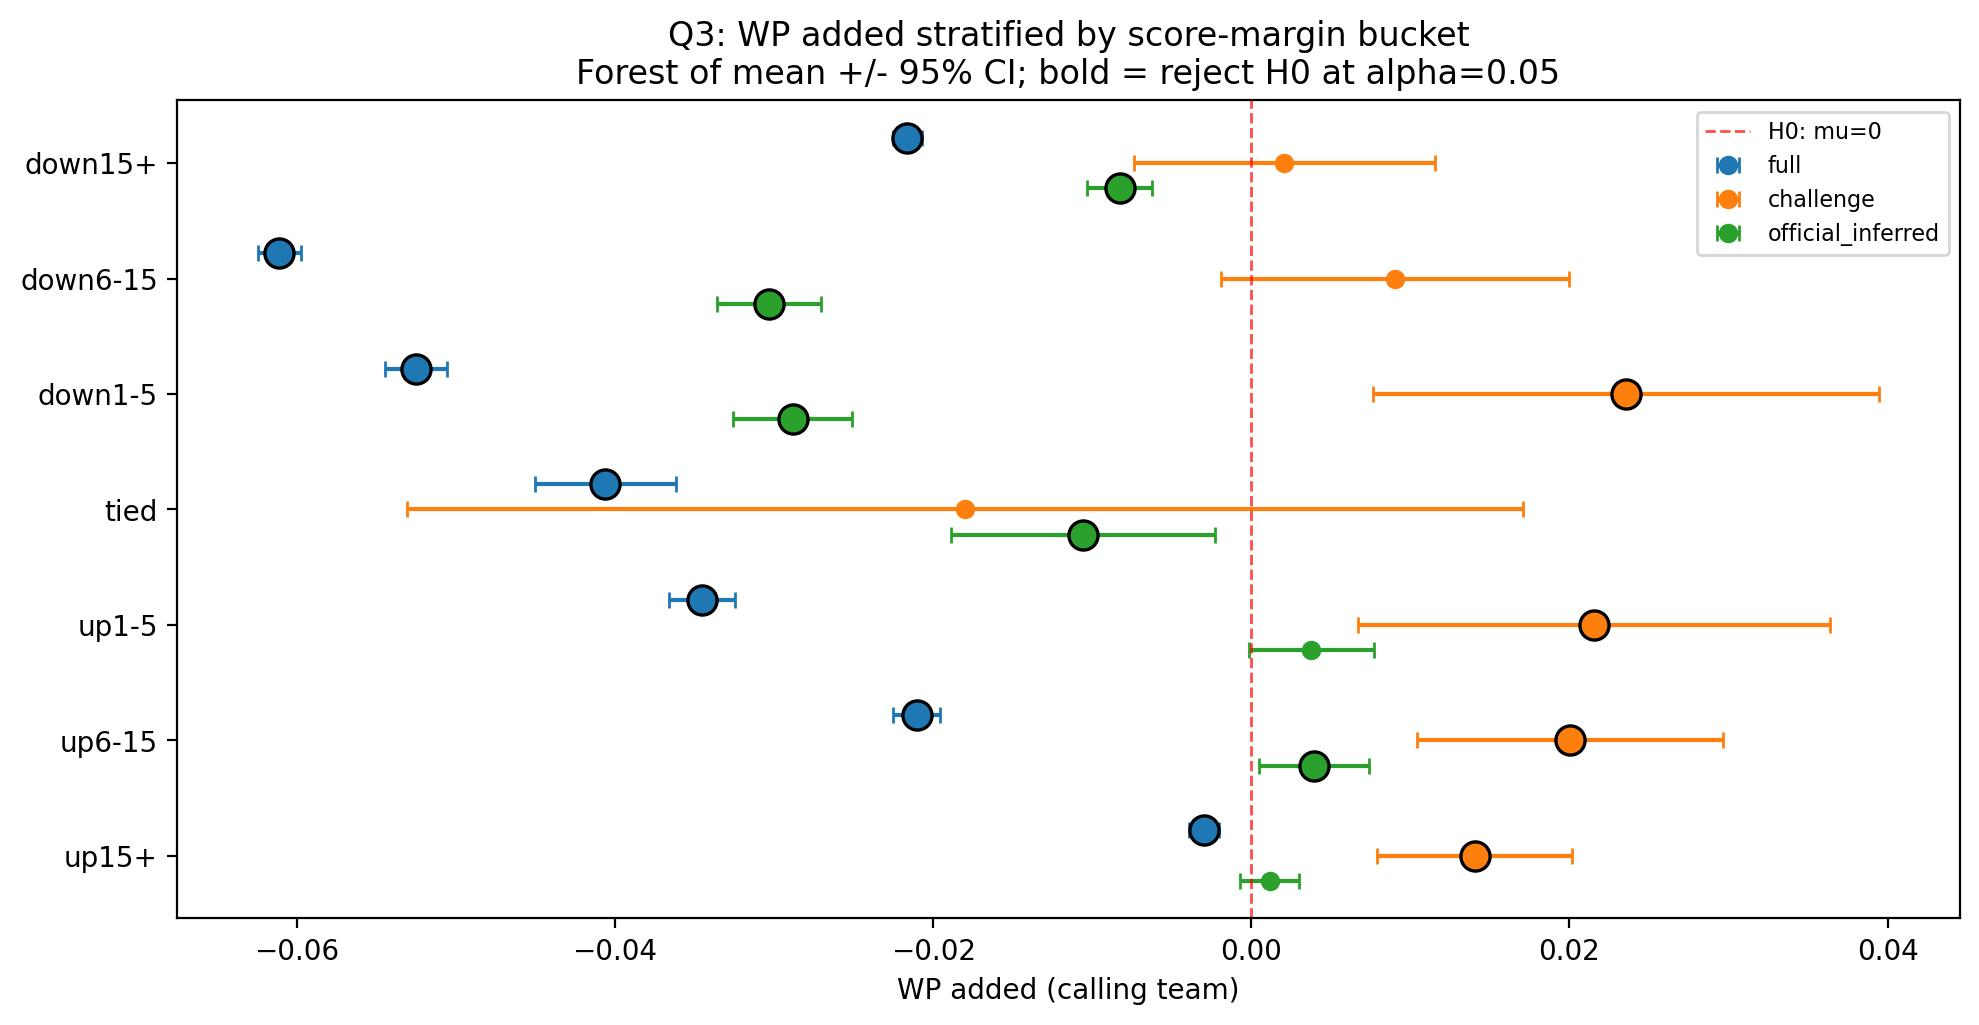
\includegraphics[width=0.85\textwidth]{figures/q3_margin.jpg}
		\caption{Q3 WP added stratified by calling-team score margin.}
		\label{fig:q3-margin}
\end{figure}

\subsection{Stratified by Game Phase}

Figure~\ref{fig:q3-time} plots Q3 by quarter, with Q4 split into early
($> 5$ min remaining) and clutch ($\leq 5$ min). Full-timeout WP cost is
roughly constant across Q1--Q3 ($-4.0$ to $-4.5$ pp) and OT ($-5.3$ pp),
but \emph{halves} in Q4-clutch ($-2.0$ pp). This is the period where
coaches are most strategic about timeout usage and where the WP model
itself becomes most informative because the score margin grows in
relative importance. TV-timeout WP cost likewise drops to zero in
Q4-clutch ($+0.0002$ pp, ns).

\begin{figure}[t]
		\centering
		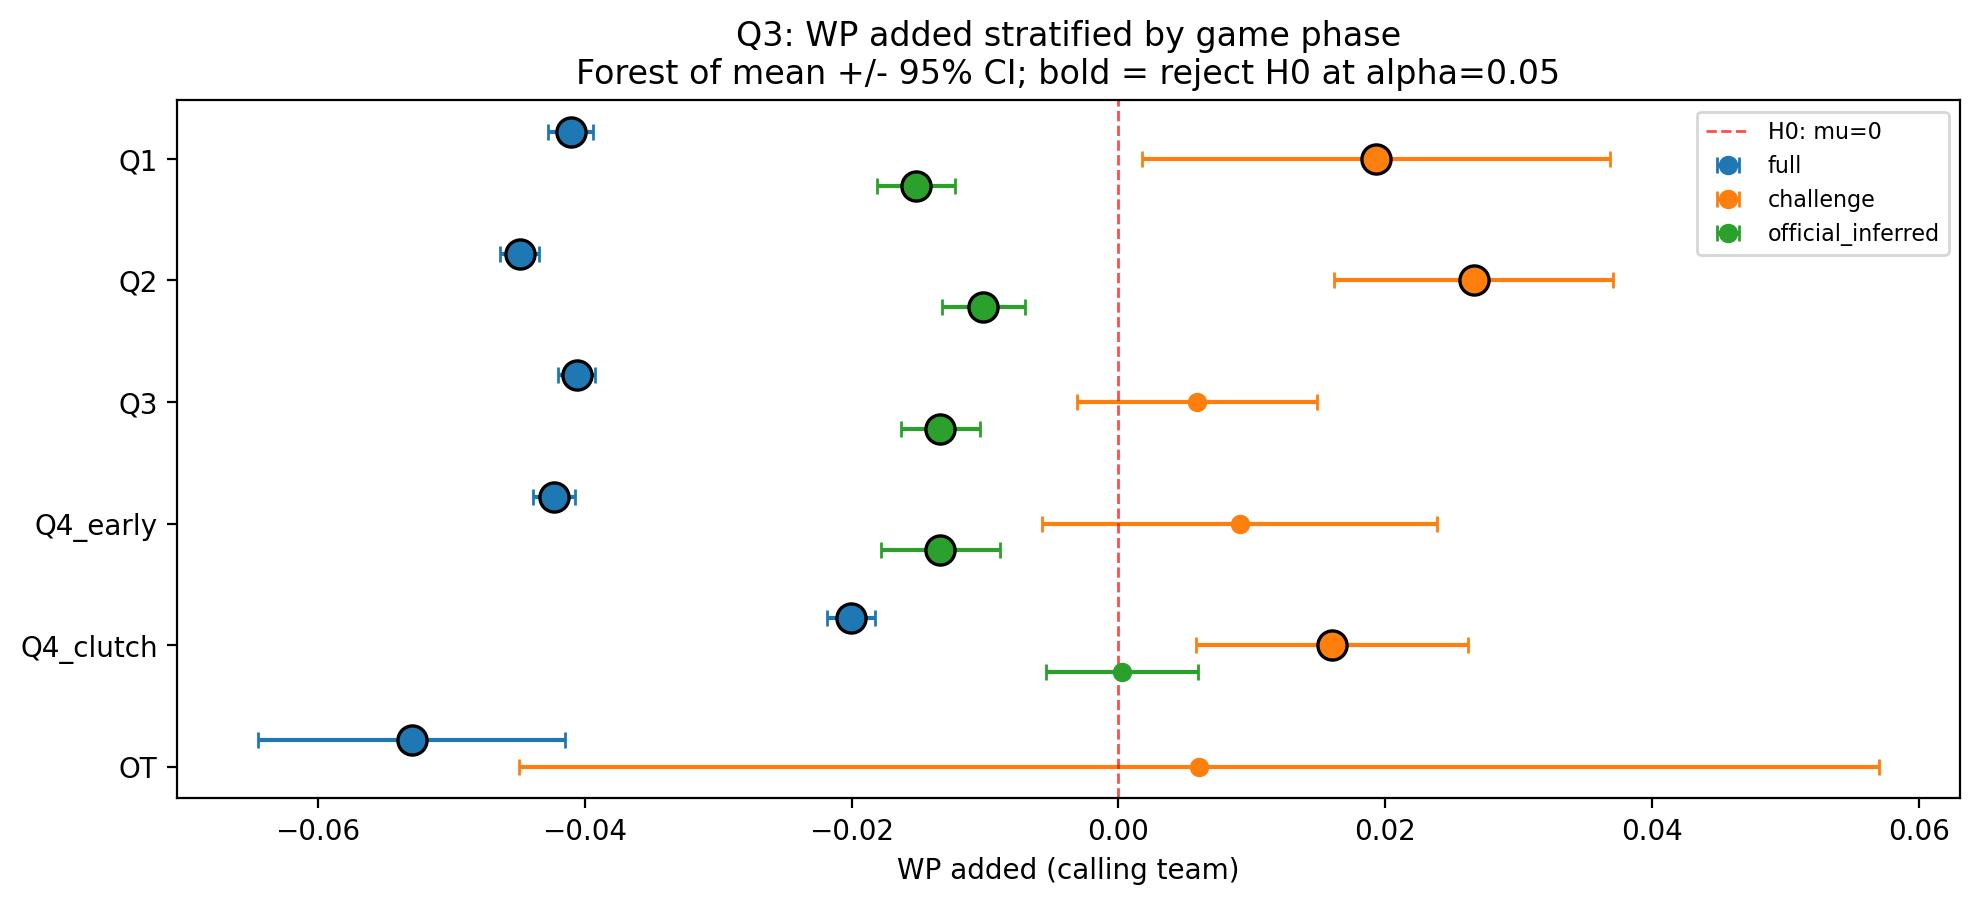
\includegraphics[width=0.85\textwidth]{figures/q3_time.jpg}
		\caption{Q3 WP added stratified by game phase.}
		\label{fig:q3-time}
\end{figure}

\subsection{Pooled Distribution of Test Statistics}

Across the four stratification schemes (overall, streak, margin, time)
and the three impact metrics, we ran $163$ stratified GLRTs and rejected
$H_0$ in $69$ ($42.3\%$). The empirical distribution of $G$ values is
strongly right-shifted relative to its asymptotic $\chi^2_1$ null
(Figure~\ref{fig:null-dist}), confirming that the rejections reflect
real signal rather than the $\sim\!5\%$ false-positive rate one would
expect under universal $H_0$.

\begin{figure}[t]
		\centering
		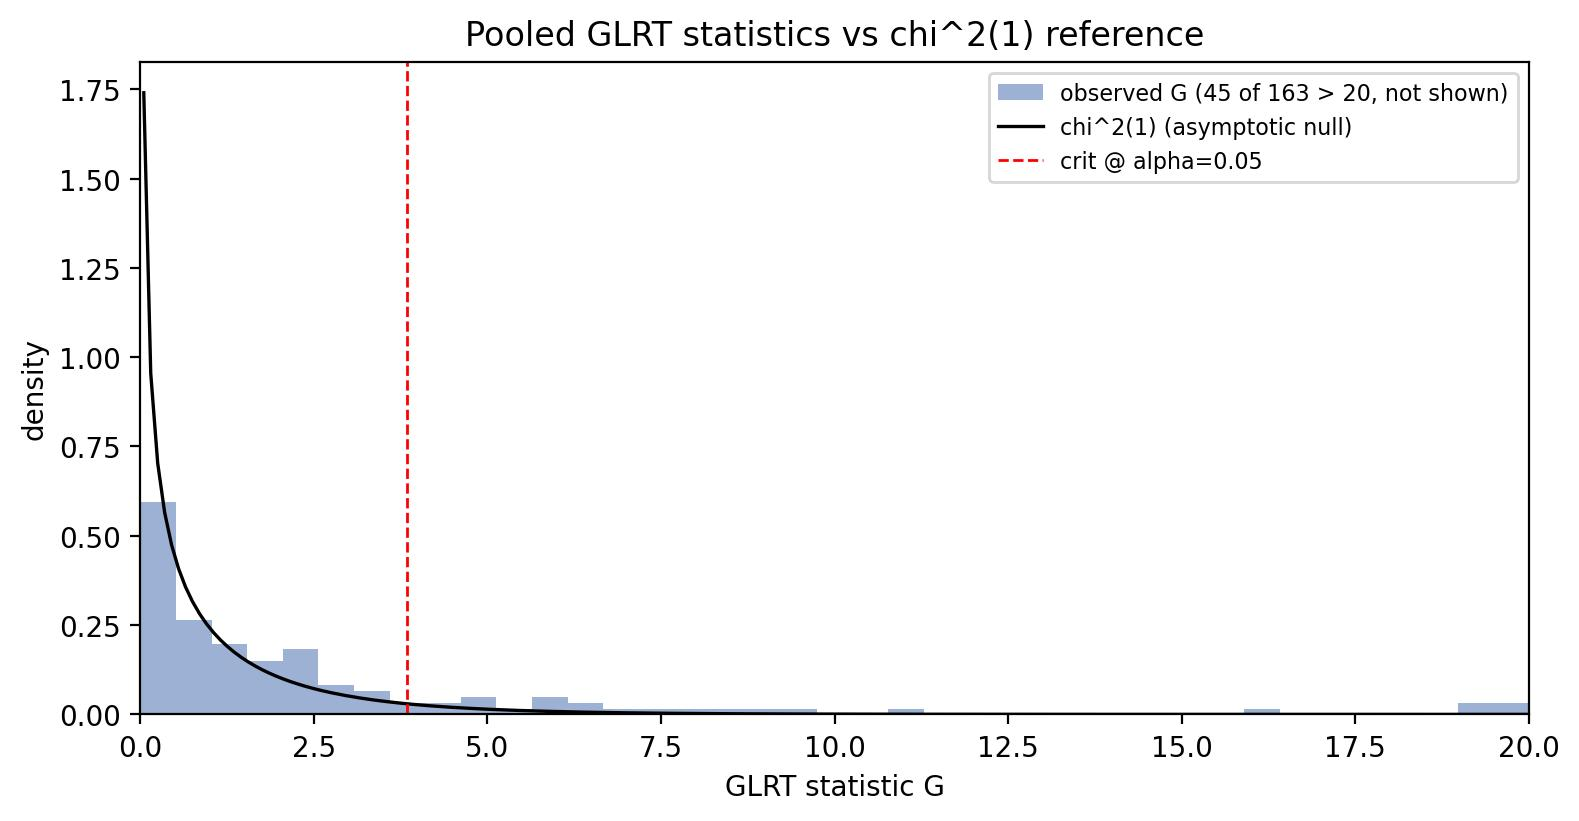
\includegraphics[width=0.7\textwidth]{figures/glrt_null_distribution.jpg}
		\caption{Pooled empirical distribution of GLRT statistics across all $163$
		stratified tests, overlaid on the asymptotic $\chi^2_1$ null reference.}
		\label{fig:null-dist}
\end{figure}

\section{Discussion}
\label{sec:discussion}

The three metrics behave differently because they absorb different sources
of variance into the null. Q1 cancels by construction in the aggregate---the
PPP-gap baseline is built precisely so that $\mathbb{E}[\,\bar X\,] = 0$
under no-effect---and only reveals signal once we stratify on a context
that the baseline does not control for. Q2 leaves opponent variance
in, which is why even the aggregate test rejects weakly. Q3 measures
WP, which is non-linear in score margin near the endgame; consequently,
the same ${\sim}1$-point swing produces drastically different WP
movements depending on game state, and the GLRT exposes this with very
high statistical power.

The signed-WP signal in Figure~\ref{fig:q3-streak} is the clearest
single result: \emph{timeouts ride momentum, they don't reverse it}.
Whether this reflects a genuine causal failure of the timeout (the
		calling team was on a hot streak and would have stayed hot anyway, but
chose to call timeout) or selection bias (coaches call timeouts at very
specific game states) cannot be answered with these between-group
GLRTs alone. The companion ``applied-causality'' report on this same
data resolves part of this ambiguity by adopting a within-game
matched-twin design, and finds that conditioning on game identity
flips the headline sign: matched-twin timeouts produce $+0.4$ pts of
recovery rather than $0$ or $-1.3$ pps of WP. The GLRT signal-detection
view here is best understood as a precise measurement of the
\emph{observed} pattern; resolving \emph{what causes it} requires the
matching design, the substitution mediator analysis, or an instrument
in the spirit of \citet{weimer2023causal}.

\paragraph{Limitations.} (i) The GLRT relies on Gaussianity of the impact
metric. Q1 and Q2 are noisy averages of point counts and are
approximately Gaussian by CLT; Q3 is an output of a logistic model and
is bounded in $[-1, 1]$, so the Gaussian assumption is violated near the
endpoints. Empirically the t-test and GLRT $p$-values agree to four
decimal places throughout, suggesting the violation is mild for $n$ this
large, but a non-parametric permutation test would be a robust check.
(ii) The $163$ tests are not independent (the same events appear in
multiple stratifications) so a Bonferroni or Benjamini--Hochberg
correction would be conservative; we report uncorrected $p$-values.
(iii) The TV-timeout cohort is rulebook-inferred rather than labeled,
with F1 $\approx 0.9$ in the validation era, so the
\texttt{official\_inferred} effects should be read as a lower bound on
the true mandatory-timeout effect.

\paragraph{Future work.} The natural next step is to replace the
unconditional null in Equation~\ref{eq:hyp} with a counterfactual null
that accounts for game state---e.g., comparing each timeout to a
matched non-timeout possession in the same game, and applying the
GLRT to the paired difference. This converts the GLRT into a
within-pair causal estimator and inherits both the variance reduction of
matching and the asymptotic distribution theory of the GLRT.

\acks{N/A}

\newpage

\bibliography{references}

\end{document}
